\section{Vorlesung 18.05.2017}

\subsection{Dynamische Systeme} % FIXME

\subsubsection{Kontinuierliche dynamische Systeme}

\begin{description}
    \item[Dynamisches System] Differentialgleichung \quad $ \dot{x} = f(x) $
    \item[Fixpunkte] $ \dot{x} = 0 \quad f(\hat{x}) = 0 $
\end{description}

\paragraph{Stabilität von Fixpunkten}
\begin{itemize}
    \item durch Linearisierung $ f(x) = f(\hat{x}) + J(\hat{x}) (x - \hat{x}) + \text{Rest} $
    \item Eigenwerte $ \lambda_1 \dots \lambda_n $ \quad ($ n $ Variablen)
        \begin{itemize}
            \item $ \Re(\lambda_i) < 0 $ \quad stabile "`Richtung"'
            \item $ \Re(\lambda_i) > 0 $ \quad instabile "`Richtung"'
            \item "`Richtung"' \quad 1. reeller Eigenwert/Eigenvektor
            \item Ein Paar konjugiert-komplexer EW/EV $ \rightarrow $ Wirbel
        \end{itemize}
\end{itemize}

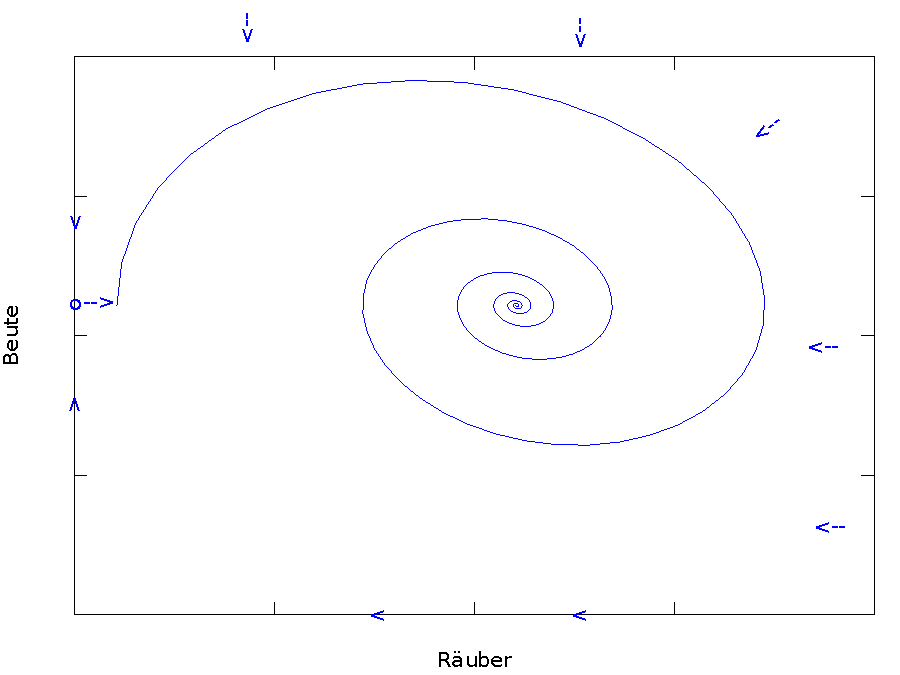
\includegraphics[width=\textwidth]{lectures/170518/pix/trajektorie_1.pdf}

\subsubsection{Diskrete dynamische Systeme}
\begin{math}
    x' = x + f(x) \\
    x' = x \; \Leftrightarrow \; f(\hat{x}) = 0 \\\\
    \epsilon := x - \hat{x} \\
    \epsilon' = x' - \hat{x} = \underbrace{x - \hat{x}}_{\epsilon} + \underbrace{f(\hat{x} + \epsilon)}_{f(\hat{x}) + J(\hat{x}) \cdot \epsilon = 0} \\ \\
    \epsilon' = \epsilon + J(\hat{x}) \cdot \epsilon = [I + J(\hat{x})] \cdot \epsilon \\
    | \Re(\mu_i) | < 1 \\\\
    \text{Eigenwerte } \mu_i \text{ von } I + J(\hat{x}) \text{ sind } 
    1 + \lambda_i \text{, wobei } \lambda_i \text{ die Eigenwerte von } 
    J(\hat{x}) \text{ sind.} \\\\
    |1 + \Re(\lambda_i)| > 1 \quad \text{instabil} \\
    |1 + \Re(\lambda_i)| < 1 \quad \text{stabil} \\\\
    \epsilon' = \epsilon + J(\hat{x}) \cdot \epsilon = [I + J(\hat{x})]
    \cdot{\epsilon} \\
    |\Re(\mu_i)| < 1
\end{math}


\subsection{Musterbildung}
